\documentclass[12pt]{article}
\usepackage[tmargin=1.25in,lmargin=1in,rmargin=1in,bmargin=1in,paper=letterpaper]{geometry}
\usepackage{amsmath,amssymb, cancel}
\usepackage{multirow,color}
\usepackage{fancyhdr,ifthen,lastpage}
\usepackage{graphicx}

\newcommand{\gen}[1]{\mathop{\left\langle #1 \right\rangle}}
\newcommand{\diff}[2][]{\mathop{\frac{d #1}{d #2}}}
\newcommand{\pdiff}[2][]{\mathop{\frac{\partial #1}{\partial #2}}}
\newcommand{\conj}[1]{\mathop{\overline{#1}}}
\newcommand{\abs}[1]{\mathop{\left\lvert #1 \right\rvert}}
\let\bb\mathbb

\begin{document}
\pagestyle{fancy}

%% HEADER %%
\lhead{ }
\rhead{Ryan Martinez }
\chead{ }

%% FOOTER %%
\lfoot{} 
\rfoot{}
\cfoot{}

\begin{center}
 {\bf Light Near a Black Hole}
\end{center}

\hrule

~

Taken from Faber 231: For $u = 1/r$ and $\theta$, so that $(r, \theta)$ is in the 
plane of the light, its velocity vector and the mass (of mass $M$) we have 
$$ \frac{d^2 u}{d\theta^2} + u = 3Mu^2.$$
Note that the units don't match up! This is because there are implicit 
$c = 1$ and $G = 1$. 
I believe the units work out to
$$ \diff[^2u]{\theta^2} + u = 3\frac{GM}{c^2}u^2.$$

We can solve this using the energy method.

We are given initial conditions as follows: The camera is a distance $R$ from the origin 
(the mass)
and looking in a direction $\phi$ from the $r$ vector. Since the equation is $\theta$ 
invariant, we may assume that the camera is at $\theta = 0$. This is given by the following 
picture:

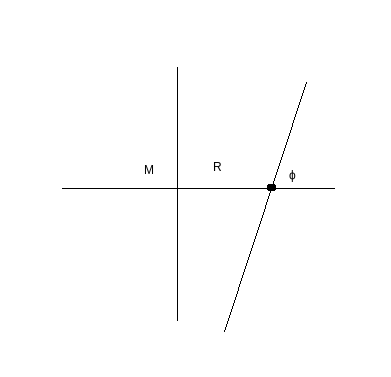
\includegraphics[width=.5\linewidth]{./geodesic.png}

Clearly $r(0) = R$ so that $u(0) = 1/r(0) = 1/R.$ Further, we see that the slope of the
line through the camera is $\tan(\phi)$ so that in Cartesian coordinates we have the 
line 
$$\cos(\phi)(y-0) - \sin(\phi)(x-R)= 0.$$
Now converting this by taking $x = r\cos(\theta)$ and $y = r \sin(\theta)$ gives 
$$r\cos(\phi)\sin(\theta) - r\sin(\phi)\cos(\theta) = R\sin(\phi).$$
Recalling the double angle for $\sin$ we see 
$$u(\theta) = \frac{1}{r} = \frac{1}{R}\frac{\sin(\phi-\theta)}{\sin(\phi)}.$$
Thus 
$$u'(0) = -\frac{1}R \frac{\cos(\phi)}{\sin(\phi)} = -\frac1R \cot(\phi).$$
We might be concerned as to what happens when $\sin(\phi) = 0 \iff \phi = 2\pi k$, $k \in \bb 
Z$. However, this is the case where the camera is either pointed directly at or away
from the mass (and so render normally). Thus, we always assume $u'(0) \in \bb R$.

Now, we can apply the Energy method in ernest.

We see that by the chain rule
$$\diff u \left[\frac12 \left(\diff[u]\theta\right)^2\right] = \diff[u]\theta 
\diff[^2u]{\theta^2} \diff[\theta]u = \diff[^2u]{\theta^2} = \frac{3GM}{c^2}u^2 - u$$
Thus,
$$\left(\diff[u]\theta\right)^2 = \frac{2GM}{c^2}u^3 - u^2 + K.$$
for $K \in \bb R.$
We can find $K$ by applying our initial conditions:
$$K = (u'(0))^2 - \frac{2GM}{c^2}u(0)^3 + u(0)^2 = \frac1{R^2}\cot(\phi)^2 - 
\frac{2GM}{c^2 R^3} + \frac1{R^2}.$$
In general, we have no cancellation, and so let's leave it as $K$.
Thus, flipping things around we have 
$$\theta = \int_{1/R}^u \frac{ds}{\sqrt{2GM s^3 / c^2 - s^2 + K}}.$$
We can solve this explicitly in special cases:
Suppose $R = 2GM/c^2$ and $\phi = \pi/2$. Then $\cot(\phi) = 0$ and 
$$K  = -\frac{2GM}{c^2}\left(\frac{c^2}{2GM}\right)^3 + \left(\frac{c^2}{2GM}\right)^2 = 0.$$
MAPLE spits out for the integral
$$\theta = 2\tan^{-1}\left(\sqrt{\frac{2GM}{c^2}u - 1}\right).$$
Solving for $r$ and remembering a few trig identities gives
$$r = \frac{GM}{c^2}(1+\cos(\theta)).$$
Which looks like for $GM/c^2 = 1$ 

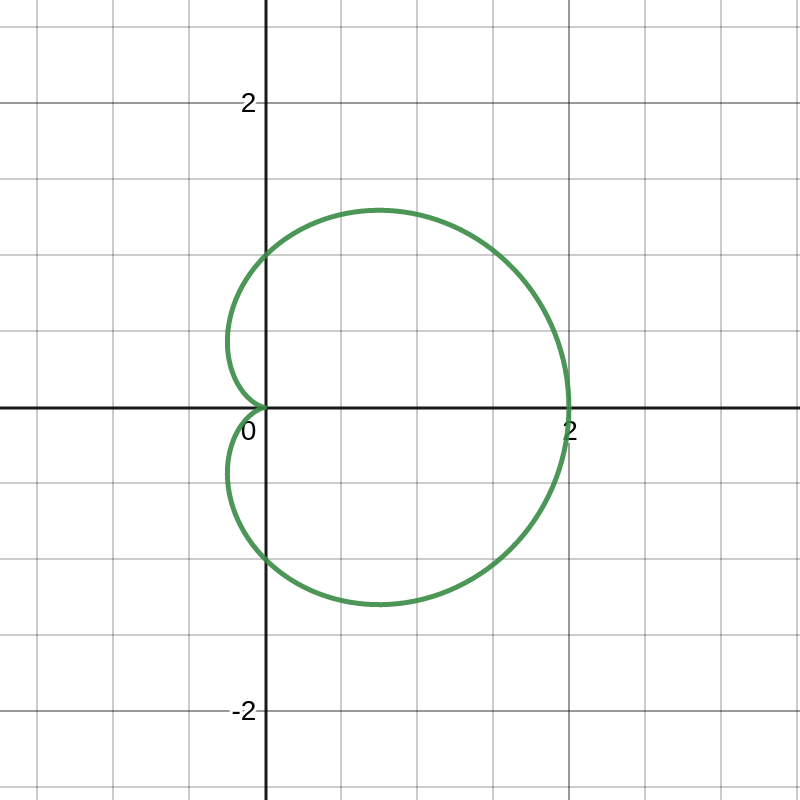
\includegraphics[width=.5\linewidth]{./schwartzschild.png}

Clearly, at this radius, the geodesic gets sucked into 0.

We could also try $R = 3GM/c^2$ and $\phi = \pi/2$. We could do it by hand, or 
simply notice that $u = c^2/(3GM)$ solves the original DE, with these initial conditions!
This is a circle of radius $3GM/c^2.$

Let's use Runge-Kutta to approximate this DE
We need to write this as 
$$\diff[y]t = f(t,y)$$
Set $$y = \left[\begin{array}{c} u\\ u' \end{array}\right]$$
So that 
$$ y' = f(y) = \left[\begin{array}{c} u'\\ u'' \end{array}\right] 
= \left[\begin{array}{c} u'\\ 3GM/c^2 u^2 - u \end{array}\right]$$
Then, for 
$$y_0 = \left[\begin{array}{c} 1/R\\ 1/R \cot(\phi) \end{array}\right],$$
$\theta_0 = 0$,
and step size $h$ (then the approximate distance traveled will be $h/u.$)
$$k_1 = f(y_n)$$
$$k_2 = f(y_n + h k_1/2)$$
$$k_3 = f(y_n + h k_2/2)$$
$$k_4 = f(y_n + h k_3)$$
$$y_{n+1} = y_n + 1/6 ~ h (k_1 + 2k_2 + 2k_3 + k_4).$$
\end{document}
